\documentclass[a4paper]{instrumentacao}

\usepackage{etoolbox}

\newtoggle{attachments}
\toggletrue{attachments}

\graphicspath{
	{../Resources/Images/}
	{../Resources/Mathematica/images/}
	{../Resources/MATLAB/images/}
}

\title{???}
\author{Rogiel Sulzbach \and Rodrigo de Castro Silveira}
\startdate{???}
\finishdate{???}
\emails{
	\emailaddress{R.J.S.}{rogiel@rogiel.com},
	\emailaddress{R.C.S.}{csilveira.rodrigo@gmail.com}
}

\resume{}
\abstract{} 
\keywords{}
\institute{}

\headertext{Extensometria}

\begin{document}
\maketitle

\chapter{Introdução}


\chapter{Metodologia Experimental}
Nestes experimentos de laboratório foi utilizado o software Wolfram Mathematica 10.4.0 da Wolfram Research, Inc. para realizar todos os cálculos no computador utilizando precisão do tipo MachinePrecision\cite{mathematica-numerial-precision} onde a precisão dos números de ponto flutuante respeitam os critérios impostos pelo processador (64 bits, precisão dupla) que implementam o padrão IEEE de ponto flutuante, possuem um "Épsilon de Máquina", o menor valor que somado a 1 retorna um valor diferente de 1, isto é, não causa arredondamento \cite{wikipedia-epsilon}, de $2^{-52}$, ou seja, na ordem de $10^{-16}$ e podem, portanto, serem desprezados perante a resolução de todos os outros instrumentos utilizados no experimento. Adicionalmente, quando possível, os cálculos foram realizados de forma simbólica com substituição numérica no final. Os scripts utilizados para cálculo estão anexados ao fim do documento, na Página \pageref{ch:attachments}.

Para a realização das simulações mecânicas, o SOLIDWORKS versão 2016 desenvolvido pela Dassault Systèmes SolidWorks Corp.

\chapter{Resultados e Discussões}

\subsection{Célula de força comercial}

Neste experimento foi levantada a função de transferência experimental para uma viga engastada utilizando uma célula de força comercial \todo{marca e outros detalhes da célula}.

Na Figura \ref{fig:celula-comercial-circuito} está apresentado o esquemático elétrico de uma ponte de Wheatstone:

\begin{figure}[H]
\center
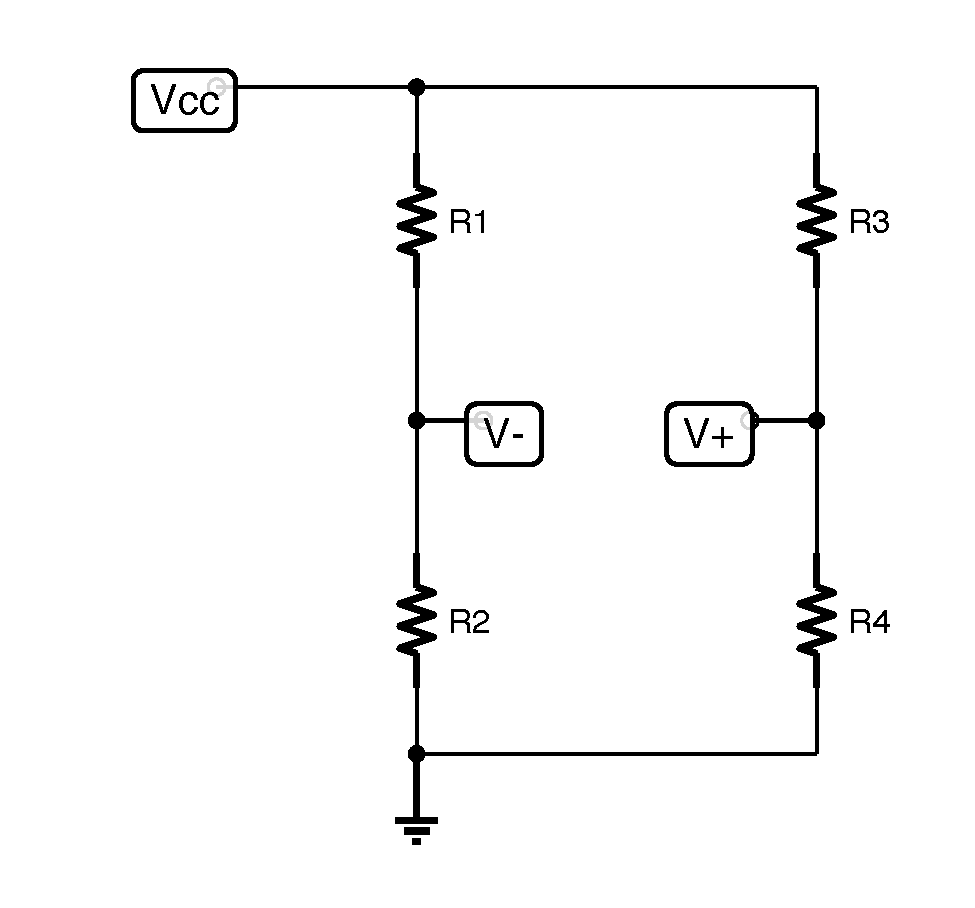
\includegraphics[width=\textwidth]{Wheatstone.pdf}
\caption{Esquemático elétrico de uma ponte de Wheatstone genérica.}
\label{fig:celula-comercial-circuito}
\end{figure}

\noindent onde os resistores $R_1$, $R_2$, $R_3$ e $R_4$ são valores de resistência elétrica que determinam o comportamento de ponte, $V_-$ e $V_+$ são os nós de saída da ponte medidos em tensão elétrica e $V_{cc}$ é a tensão elétrica de alimentação da ponte.

A função de transferência da ponte de Wheatstone proposta é dada conforme Equação \ref{eq:wheatstone-tf}:

\begin{equation}
	V_o = V_+ - V_- = \left(\dfrac{R_4}{R_4 + R_3} - \dfrac{R_2}{R_1 + R_2}\right)V_{cc}
	\label{eq:wheatstone-tf}
\end{equation}

Considerando que as condições das Equações \ref{eq:celula-comercial-cond1} e \ref{eq:celula-comercial-cond2} são válidas, então a ponte é dita estar "em equilíbrio", isto é, a saída de tensão elétrica entre $V_-$ e $V_+$ é de $OV$.

\begin{eqnarray}
	R_1 = R_4 \label{eq:celula-comercial-cond1} \\
	R_2 = R_3 \label{eq:celula-comercial-cond2}
\end{eqnarray} 

Qualquer pequena variação de resistência elétrica em qualquer um dos resistores da Figura \ref{fig:celula-comercial-circuito} que violem as condições da Equação \ref{eq:celula-comercial-cond1} e \ref{eq:celula-comercial-cond2} incorre no desequilíbrio da ponte que pode ser medido utilizando a saída em tensão elétrica.

Com isto, a ponte pode ser utilizada como circuito de condicionamento para um sistema de medição de deformação mecânica de um corpo. Na Figura \ref{fig:celula-comercial-esquema-fisico} está apresentado um esquemático físico da célula de carga comercial utilizada:

\begin{figure}[H]
\center
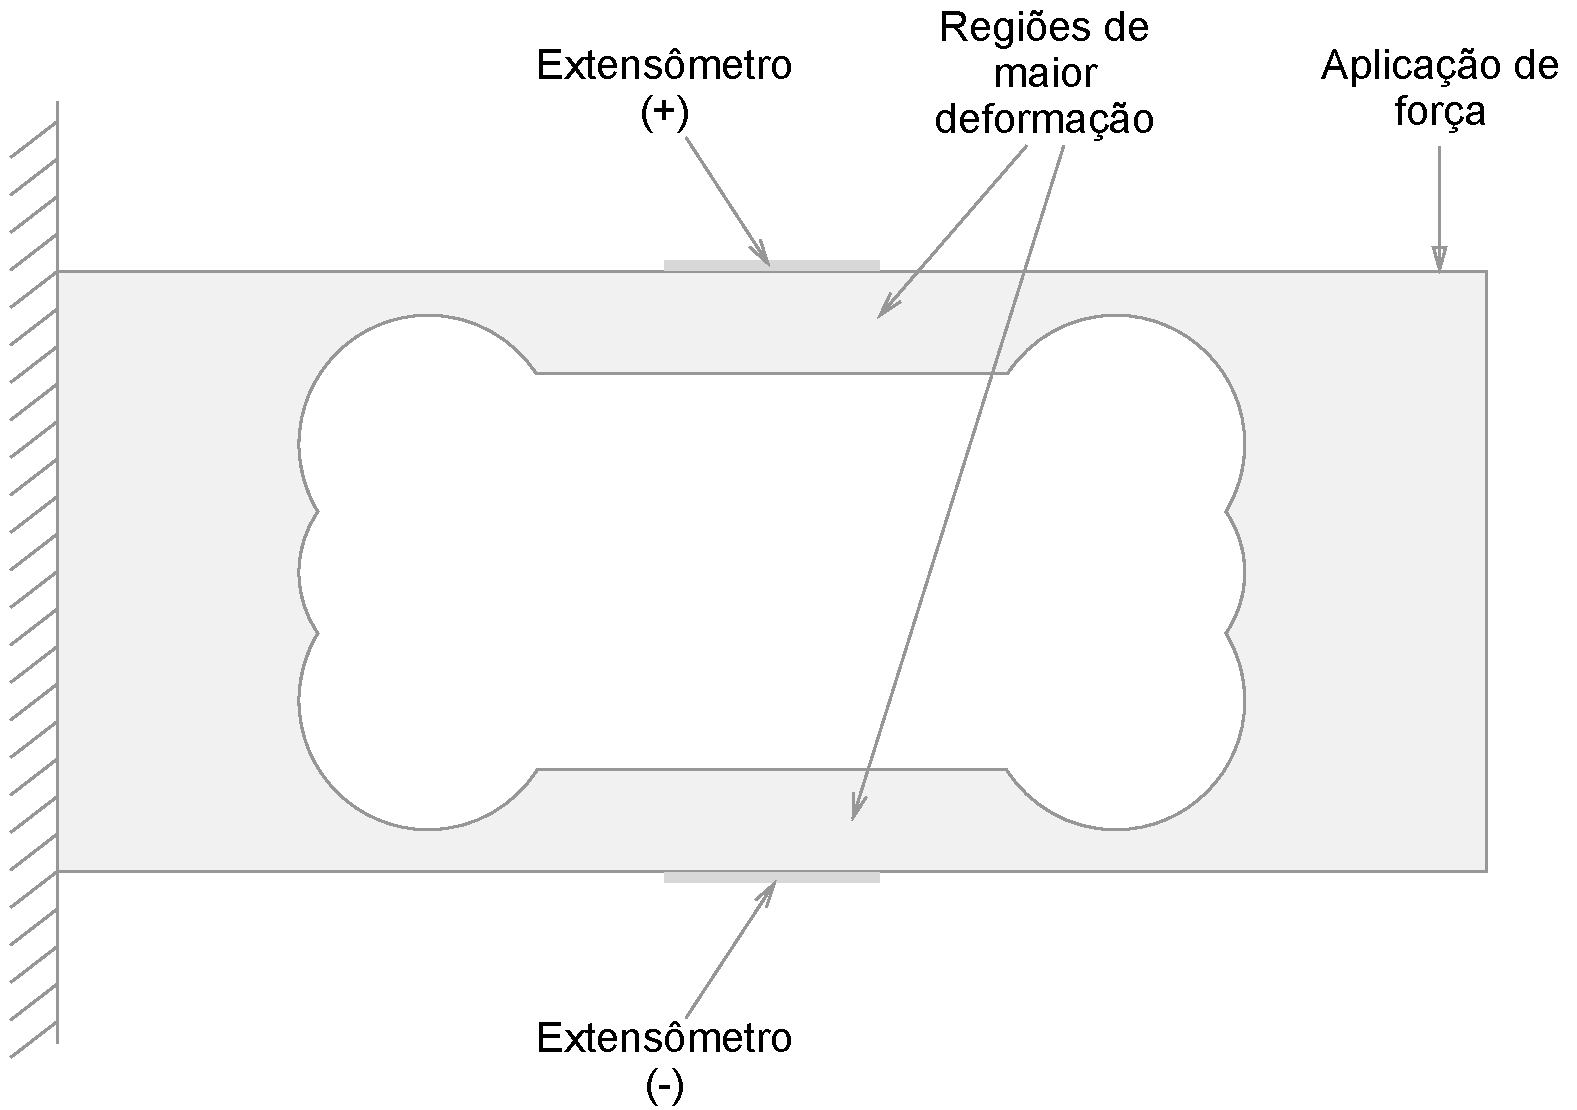
\includegraphics[width=\textwidth]{CelulaComercial.pdf}
\caption{Esquemático da construção mecânica da célula de carga comercial utilizada no experimento.}
\label{fig:celula-comercial-esquema-fisico}
\end{figure}

\noindent onde o extensômetro $(+)$ indica uma deformação positiva (alongamento) e o extensômetro $(-)$ indica uma deformação negativa (compressão).

Portanto, é possível utilizar esta construção como forma de medir deformações que a viga proposta esteja submetida. É comum utilizar 3 formas distintas de medição utilizando extesômetros e a ponte de Wheatstone.

\todo{continuar}

\subsection{Célula de força não-comercial}

A célula de força não comercial utilizada possui a configuração dada na Figura \ref{fig:celula-nao-comercial-desenho}:

\begin{figure}[H]
\center
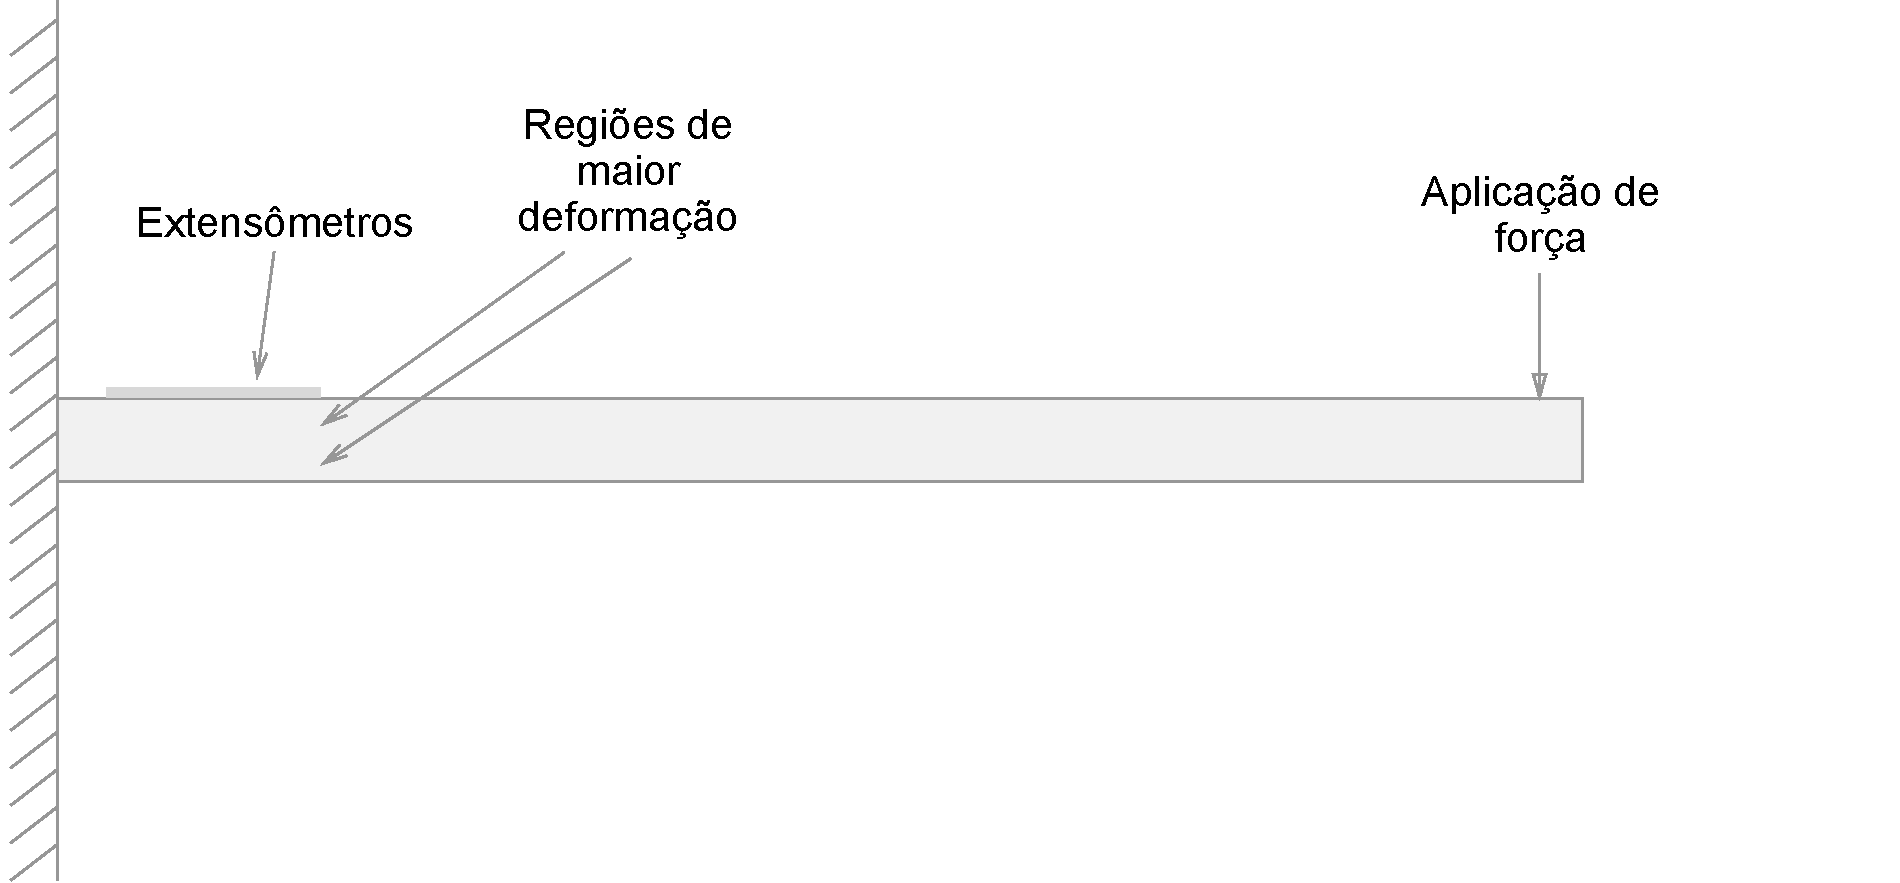
\includegraphics[width=\textwidth]{CelulaNaoComercial.pdf}
\caption{Esquemático da construção mecânica da célula de carga não-comercial utilizada no experimento.}
\label{fig:celula-nao-comercial-desenho}
\end{figure}

\noindent onde o extensômetro $(+)$ indica uma deformação positiva (alongamento) e o extensômetro $(-)$ indica uma deformação negativa (compressão).

Ao contrário da célula comercial, esta nao possui a ponte pré-calibrada e, portanto, se fez necessário que a ponte fosse calibrada e ajustada para obter o resultado desejado. De acordo com a especificação dos extensômetros (modelos e fabricantes não estavam explícitos sobre a construção, logo, não foi possível comparar com os valores fornecidos pelo fabricante). Havia, contudo, uma marcação indicando o valor de resistência nominal do extensômetro.


\chapter{Conclusões}



\newpage
\begin{thebibliography}{9}
\bibitem{mathematica-numerial-precision} \url{https://reference.wolfram.com/language/tutorial/NumericalPrecision.html}, acessado em 26 de abril de 2016
\bibitem{wikipedia-epsilon} \url{https://en.wikipedia.org/wiki/Machine_epsilon}, acessado em 26 de abril de 2016
\bibitem{livro-texto}  Balbinot, Alexandre; Brusamarello, Valner J., Instrumentação e Fundamentos de Medida - Vol.1 - 2ª Ed. Rio de Janeiro: LTC, 2014.
\bibitem{daq-specifications} NI USB-6009 -- DEVICE SPECIFICATIONS, \url{http://www.ni.com/pdf/manuals/375296a.pdf}, acessado em 3 de maio de 2016
\bibitem{daq-user-guide} NI USB-6009 -- USER GUIDE, \url{http://www.ni.com/pdf/manuals/371303n.pdf}, acessado em 3 de maio de 2016
\bibitem{datasheet-lm7805} Datasheet oferecido pelo fabricante do regulador de tensão LM7805CV, disponível em \url{http://www.datasheetlib.com/datasheet/221840/l7805cv_stmicroelectronics.html}.
\bibitem{datasheet-ina126} Datasheet oferecido pelo fabricante amplificador de instrumentação INA126, disponível em \url{http://www.ti.com/lit/ds/symlink/ina126.pdf}.

\end{thebibliography}

\iftoggle{attachments}{
	\chapter*{Anexos}
	\label{ch:attachments}
	\section{Mathematica}
	
}

\end{document}
